\chapter{Identification of do queries via LDEN
diagrams}
\label{ch-iden-LDEN}

The most general way to decide whether a do query for
a particular DAG is identifiable, is by using Pearl's
Do Calculus rules (see Chapter \ref{ch-do-calc}). However, those rules are fairly 
complicated and therefore difficult to automate.


We contend that by analyzing any DAG {\it symbolically} using 
SCuMpy (see Ref.\cite{scumpy}), one can decide rigorously 
whether a
do query for that DAG is identifiable or not. Hence, SCuMpy
allows us, {\it if we have a single specific DAG in mind}, to bypass and supplant, in an automated 
fashion, the Do Calculus rules.

SCuMpy uses
LDEN diagrams (a.k.a. linear SCM, see Chapter \ref{ch-linear-sys}) whereas
the Do Calculus rules are for general bnets.
However, the answer to the question
of whether a do query is identifiable
for a particular DAG,
only depends on the DAG,
so it is independent of whether
the DAG came from an LDEN diagram, or from
the more general corresponding bnet.


In this chapter,
we will briefly summarize the results
presented in the
Jupyter notebook entitled \enquote{unconfounded-children} in SCuMpy (Ref
.\cite{scumpy}). See that notebook
for more details.

\begin{figure}[h!]
\centering
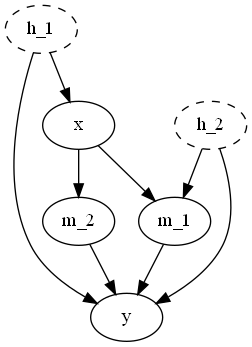
\includegraphics[width=2in]
{iden-LDEN/uncon-children.png}
\caption{LDEN diagram for which 
the query $P(y|do(x))$
is  known to be identifiable.
External root nodes $\rveps_\rva$ 
pointing into each node $\rva$,
are left implicit.
The path coefficients (a.k.a
arrow gains)
are not shown either. 
For any two nodes $\rva, \rvb$,
these gains
 are denoted
   by $\alp_{\rvb|\rva}$
for an arrow $\rva\rarrow \rvb$.}
\label{fig-uncon-children}
\end{figure}

Consider the LDEN diagram of 
Fig.\ref{fig-uncon-children}.
This DAG does not satisfy either
the backdoor or frontdoor criteria, but the query
$P(y|do(x))$ is still known to be identifiable for this DAG.


For the 
LDEN diagram of 
Fig.\ref{fig-uncon-children}, 
SCuMpy gives the following 
covariance between nodes $\rvx$
and $\rvy$:
\beq
\left\langle\underline{x}, \underline{y}\right\rangle=
\left\{\begin{array}{l}
\alpha_{\underline{x}|\underline{h_1}} \sigma^2_{\underline{\epsilon}_{\underline{h_1}}} \left(\alpha_{\underline{m_1}|\underline{x}} \alpha_{\underline{x}|\underline{h_1}} \alpha_{\underline{y}|\underline{m_1}} + \alpha_{\underline{m_2}|\underline{x}} \alpha_{\underline{x}|\underline{h_1}} \alpha_{\underline{y}|\underline{m_2}} + \alpha_{\underline{y}|\underline{h_1}}\right)
\\ + \sigma^2_{\underline{\epsilon}_{\underline{x}}} \left(\alpha_{\underline{m_1}|\underline{x}} \alpha_{\underline{y}|\underline{m_1}} + \alpha_{\underline{m_2}|\underline{x}} \alpha_{\underline{y}|\underline{m_2}}\right)
\end{array}
\right.
\eeq

Suppose we amputate, 
from the LDEN diagram of 
Fig.\ref{fig-uncon-children}, all 
arrows entering node $\rvx$
(for this example,
that means amputating the arrow
$\rvh_1\rarrow \rvx$).
Such an amputation is demanded by the definition of
the do query $P(y|do(x))$, 
Then SCuMpy gives instead:

\beq
\left\langle\underline{x}, \underline{y}\right\rangle=
 \sigma^2_{\underline{\epsilon}_{\underline{x}}} \left(\alpha_{\underline{m_1}|\underline{x}} \alpha_{\underline{y}|\underline{m_1}} + \alpha_{\underline{m_2}|\underline{x}} \alpha_{\underline{y}|\underline{m_2}}\right)
\eeq
so

\beq
\pder{\rvx}{\rvy}
=\frac{\av{\rvx, \rvy}}{\av{\rvx, \rvx}}=
\alpha_{\underline{m_1}|\underline{x}} \alpha_{\underline{y}|\underline{m_1}} + \alpha_{\underline{m_2}|\underline{x}} \alpha_{\underline{y}|\underline{m_2}}
\eeq

Note that upon amputating
the arrows entering $\rvx$,
the covariance $\av{\rvx, \rvy}$
becomes independent of the 
hidden (i.e., unobserved)
variables $\rvh_1, \rvh_2$.
Thus, the do query
$P(y|do(x))$ is identifiable,
because it doesn't 
depend on unobserved quantities.



